\subsection{Open Collaboration in the Classroom}
\label{opencollaborationintheclassroom}

From preliminary work including personal engagement in an open collaboration project and individual assignments, one main goal of the class is to produce a relevant collective report with no {\it ex-ante} guidelines and with self-organization as the default more. Instructors act as ``benevolent dictators" only when required or if extensive discussion are likely the impede to finish the report on time. We report on the main (self-)organization steps for this report.

\begin{enumerate}
  \item collective report topic brainstorming {\bf (self-organized)} : recall the date and what has triggered a change in the syllabus
  \item decision to design a survey {\bf (instructors)} : by the instructors
  \item survey design {\bf (self-organized)} : question design (one by student) + categories
  \item survey answering {\bf (instructors)} : everyone had to take the survey within a precise time window (recall it)
  \item survey analysis {\bf (instructors)} :  each of us was asked to perform an analysis of her own proposed question(s).
  \item report Latex format {\bf (instructors + self-organized)} : choice for Latex by the instructors
  \item learning Latex {\bf (self-organized)} : no crash course $\rightarrow$  learning by doing (c.f. next point)
  \item producing a first chunk {\bf (self-organized)} :
  \item Latex compilation {\bf (self-organized)} : not even necessary  
  \item group formation to handle parts of the report {\bf (self-organized)}
  \item production by groups {\bf (self-organized)} : drafts on Google Docs
  \item peer-review {\bf (self-organized)} : group rotation
  \item editing harmonization {\bf (self-organized)} : few rules (use ``we", present tense by default)
\end{enumerate}


\begin{figure}[ht!]
\centering
%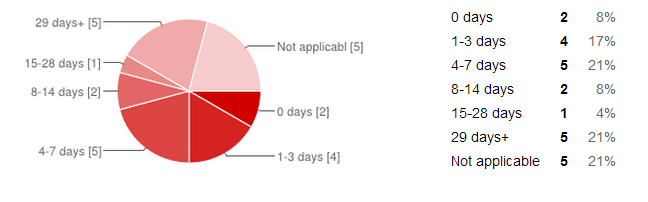
\includegraphics[width=90mm]{chapters/img/lurking_response.png}
\caption{Network of survey topic organization and Progressive merging}
\label{overflow}
\end{figure}



\mysubsubsection{Other patterns of self-organization :} 

\begin{itemize}
  \item committer rights on github repo granted to volunteers.
  \item Various communication tools used on a best match way : Etherpad, Google Docs, Google Forms. Make a list of various ad-hoc documents.
  \item Instructors become increasingly community managers
\end{itemize}

